\documentclass[12pt]{article}
\usepackage{light}

\hidesolutions
%\showsolutions

\newcommand{\edge}[2]{#1\text{---}#2}
\newcommand{\mfigure}[3]{\bigskip\centerline{\resizebox{#1}{#2}{\includegraphics{#3}}}\bigskip}
\newcommand{\eqdef}{\mathbin{::=}}

\begin{document}

\recitation{6}{September 24, 2014}

%%%%%%%%%%%%%%%%%%%%%%%%%%%%%%%%%%%%%%%%%%%%%%%%%%%%%%%%%%%%%%%%%%%%%%%%%%%%%%%
%\insolutions{
%\stamp
\section{Graph Basics}

Let $G = (V,E)$ be a graph. Here is a picture of a graph.
\begin{center}
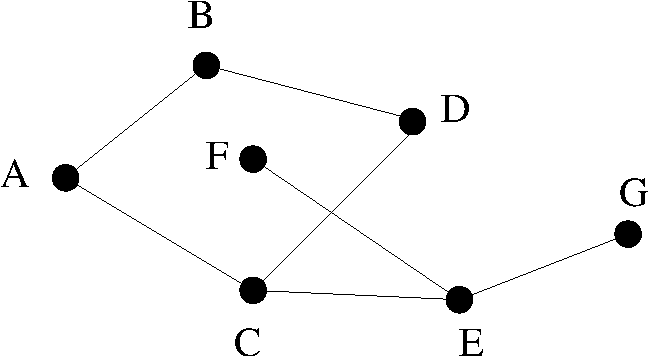
\includegraphics[height=1.75in]{example}
\end{center}
Recall that the elements of $V$ are called vertices, and those of $E$
are called edges. In this example the vertices are $\set{A, B, C, D,
  E, F,G}$ and the edges are $$\set{\edge{A}{B}, \edge{B}{D},
  \edge{C}{D}, \edge{A}{C}, \edge{E}{F}, \edge{C}{E}, \edge{E}{G}}.$$

Deleting some vertices or edges from a graph leaves a {\em subgraph}.
Formally, a subgraph of $G = (V, E)$ is a graph $G' = (V', E')$ where
$V'$ is a nonempty subset of $V$ and $E'$ is a subset of $E$.  Since a
subgraph is itself a graph, the endpoints of every edge in $E'$ must
be vertices in $V'$. For example, $V' = \set{A,B,C,D}$ and $E' =
\set{\edge{A}{B},\edge{B}{D},\edge{C}{D}, \edge{A}{C}}$ forms a
subgraph of $G$.

In the special case where we only remove edges incident to removed
nodes, we say that $G'$ is the {\em subgraph induced on $V'$} if $E' =
\{( \edge{x}{y}| x,y \in V' {\rm ~and~} \edge{x}{y} \in E \}$.  In
other words, we keep all edges unless they are incident to a node not
in $V'$. For instance, for a new set of vertices $V'=\set{A,B,C,D}$,
the induced subgraph $G'$ has the set of edges $E'=
\set{\edge{A}{B},\edge{B}{D},\edge{C}{D}, \edge{A}{C}}$.

\section{Problem 1}
An undirected graph $G$ has \term{width} $w$ if the vertices can be
arranged in a sequence
%
\[
v_1,\ v_2,\ v_3,\ \ldots,\ v_n
\]
%
such that each vertex $v_i$ is joined by an edge to at most $w$
preceding vertices.  (Vertex $v_j$ \textit{precedes} $v_i$ if $j <
i$.)  Use induction to prove that every graph with width at most $w$
is $(w + 1)$-colorable.

(Recall that a graph is \textit{$k$-colorable} iff every vertex can be
assigned one of $k$ colors so that adjacent vertices get different
colors.)


\solution{We use induction on $n$, the number of vertices.  Let $P(n)$
be the proposition that every graph with width $w$ is $(w+1)$
colorable.

\noindent \textit{Base case:} Every graph with $n = 1$ vertex has
width 0 and is $0 + 1 = 1$ colorable.  Therefore, $P(1)$ is true.

\noindent \textit{Inductive step:} Now we assume $P(n)$ in order to
prove $P(n+1)$.  Let $G$ be an $(n+1)$-vertex graph with width $w$.
This means that the vertices can be arranged in a sequence
%
\[
v_1, v_2, v_3, \ldots, v_n, v_{n+1}
\]
%
such that each vertex $v_i$ is connected to at most $w$ preceding
vertices.  Removing vertex $v_{n+1}$ and all incident edges gives a
graph $G'$ with $n$ vertices and width at most $w$.  (If original
sequence is retained, then removing $v_{n+1}$ does not increase the
number of edges from a vertex $v_i$ to a preceding vertex.)  Thus,
$G'$ is $(w+1)$-colorable by the assumption $P(n)$.  Now replace
vertex $v_{n+1}$ and its incident edges.  Since $v_{n+1}$ is joined by
an edge to at most $w$ preceding vertices, we can color $v_{n+1}$
differently from all of these.  Therefore, $P(n+1)$ is true.

The theorem follows by the principle of induction.}

\section{Problem 2}
A {\bfseries planar graph} is a graph that can be drawn without any edges crossing.
\begin{enumerate}
\item First, show that any subgraph of a planar graph is planar.
\solution{
The edge set of any subgraph will be a subset of the set of edges in the original planar graph. This means that since edges in the original graphs do not cross, edges in a subset of the original set of edges also do not cross.
}

\item Also, any planar graph has a node of degree at most 5. Now, prove by induction that any graph can be colored in at most 6 colors.
\solution{
We prove by induction. First, let $n$ be the number of nodes in the graph. Then define
\[P(n)=\text{Any planar graph with $n$ nodes is 6-colorable.}\]

\noindent \textit{Base case, $P(1)$:} Every graph with $n = 1$ vertex is 6-colorable. Clearly true since it's actually 1-colorable.

\noindent \textit{Inductive step, $P(n) \rightarrow P(n+1)$:} Take a graph $G$ with $n+1$ nodes. Then take a node $v$ with degree at most 5 (which we know exists because we know any planar graph has a node of degree $\leq 5$), and remove it. We know that the induced subgraph $G'$ formed in this way has $n$ nodes, so by our inductive hypothesis, $G'$ is 6-colorable. But $v$ is adjacent to at most 5 other nodes, which can have at most 5 different colors between them. We then choose $v$ to have an unused color (from the 6 colors), and as we have constructed a 6-coloring for $G$, we are done with the inductive step.

\noindent Because we have shown the base case and the inductive step, we have proved
\[\forall n \in \mathbb{Z}_+:P(n)\]
(Note: $\mathbb{Z}_+$ refers to the set of positive integers.)
}
\end{enumerate}

%%%%%%%%%%%%%%%%%%%%%%%%%%%%%%%%%%%%%%%%%%%%%%%%%%%%%%%%%%%%%%%%%%%%%%%%%%%%%%%

\end{document}
